\documentclass{article}
\usepackage[utf8]{inputenc}
\usepackage[margin=1.2in]{geometry}
\usepackage{amsmath,amssymb}
\usepackage{graphicx}
\usepackage{esvect}
\usepackage{fancyhdr}
\usepackage{amsthm}
\usepackage{tikz}
\usepackage{color}   %May be necessary if you want to colour links
\usepackage{hyperref}
\usepackage{lastpage}
\usepackage{pifont}
\usepackage{mathtools}


\hypersetup{
    colorlinks=true, %set true if you want colored links
    linktoc=all,     %set to all if you want both sections and subsections linked
    linkcolor=blue,  %choose some color if you want links to stand out
}
% \pagestyle{plain}
% \pagestyle{fancy}
% % \fancyhf{}
% \cfoot{}
% \fancyfoot[R]{Page \thepage\ of }

\theoremstyle{plain}
\newtheorem{theorem}{Theorem}
\newtheorem{proposition}{Proposition}


\theoremstyle{definition}
\newtheorem{definition}{Definition}
\newtheorem{example}{Example}

\theoremstyle{remark}
\newtheorem{rem}{Remark}



% Custom Commands 
\newcommand{\R}{\mathbb{R}}


\title{Differential Geometry of Surfaces}
\author{Pankaj Ghodla }
% \date{January 2021}

\begin{document}
\maketitle
\tableofcontents

\newpage


\section{Introduction}
In this section, we will introduce some of the basic definition of curves and surfaces.
\subsection{Curves}
Intuitively, A curves can be thought as the trace of a moving particle in the space. Mathematical, a curves is defined to be the image of a function, \( \gamma: U \rightarrow \R^n \), where U \( \subset \R \)..

\begin{definition}[Parametrised curve]
    A \textbf{parametrised curve} in \( \R^n \) is a smooth function \( \gamma: U \rightarrow \R^n \), where U \( \subset \R \).
\end{definition}
Throughout, this report we will assume that smoothness mean \( \text{C}^\infty \), i.e. the function is differentiable infinitely many times.

\begin{definition}[Regular curve]
    Let \( \gamma: U \rightarrow \R^n \) be a curve. It is called regular if its derivative is non-vanishing, i.e. \( \left\lVert  \gamma^\prime(t) \right\rVert \neq 0 \), \( \forall \in U \).
\end{definition}

There are many different ways to parametrise a curve, e.g. \( \gamma(t) = (t, t^2)\) and \( \tilde{\gamma}(t) = (t^2, t^4)\). However, only one of these curve is regular, which is \( \gamma(t) \). Moreover, there are many different ways to parametrise a curves such that all the parametrisations are regular.

\begin{definition}[Unit speed curve]
    Let \( \gamma: U \rightarrow \R^n \) be a curve. It is called unit-speed, if \( \left\lVert  \gamma^\prime(t) \right\rVert = 1 \), \( \forall \in U \).
\end{definition}
We will see later on that a lot of the formulas and results relating to curves take on a much simpler form when the curve is unit-speed, e.g. curvature of a unit-speed curve, see definition \ref{definition: Curvature of a curve}, is just the norm of it's second derivative.

\begin{proposition}
    A parametrised curve is unit-speed if and only if it is regular.
\end{proposition}
{\color{red} proof ??}

{\color{red} Explain in more detail why curvature is defined in the following manner: }
\begin{definition}[Curvature of a curve] \label{definition: Curvature of a curve}
    Let \( \gamma: U \rightarrow \R^n \) be a unit-speed curve. The curvature at point \( \gamma(t) \) is defined as \[ \kappa(t) = \left\lVert \gamma^{\prime\prime} \right\rVert  \]
\end{definition}

These are all the definitions and results about curves that we need to know to understand this report.
\subsection{Surfaces}
Intuitively, a surface is a subset of \( \R^3 \) that looks like a \( \R^2 \)  in the neighbourhood of any given point, e.g. the surface of the Earth is spherical; however, it appear to be a flat plane(\( \R^2 \)) to an observer on the surface.

\begin{definition}[Diffeomorphism]
    if \( f: U \rightarrow W \) is continuous, bijective, and smooth, and if its inverse maps \( f^{-1}: W \rightarrow U\) is also continuous and smooth, then f is called a diffeomorphism and \(U\) and \(W\) are called diffeomorphic.
\end{definition}

\begin{definition}[Regular Surface]
    A subset of \( \R^3 \) is a regular surface, if every point P \( \in S \), there exists a open set \( U \text{ in } \R^2\) and an open set \( W \text{ in } \R^3\) containing P such that \( S \cap W\) is diffeomorphic to \(U\).
\end{definition}
Therefore, a surface is collection of diffeomorphisms, \( \sigma: U \rightarrow S \cap W \), which we call regular surface patches.

\begin{definition}[Reparametrisation of surface patches]
    Let \( \sigma: U \rightarrow S\) and \( \tilde{\sigma}: \tilde{U} \rightarrow S\) be surface patches for a surface S, then \( \tilde{\sigma} \) is called a reparametrisation of \( \sigma \) if there exists a map, \( \Phi: \tilde{U} \rightarrow U \), which is smooth and bijective with smooth inverse, \( \Phi^{-1}: U \rightarrow \tilde{U} \).
\end{definition}

\begin{definition}[Tangent space]
    Let \(S\) be a regular surface. The \textbf{tangent plane} to \(S\) at the point \( p \in S\) is the set of all initial velocity vectors of regular curves in \(S\) with initial position \(p\), i.e \[ T_pS = \{ \gamma^\prime(0) | \gamma \text{ is a regular curve in S with }\gamma(0) = p\} \]
\end{definition}

These are all the definitions about surfaces that we need to understand this report.

\section{First Fundamental Form}
In this section, we will define one of the most important object that lets us compute lengths, angles and areas on surface. It is called the \textbf{first fundamental form}.

\begin{definition}[The fundamental form]
    The \textbf{first fundamental form} is the restriction of the inner product of the ambient space(\(\R^3\)) to the tangent space(\( T_pS\)) at point \( p \in S\). The first fundamental form is denoted by \( \mathbf{I} \), \[ \mathbf{I}(x,y) = \left\langle x,y\right\rangle  \], where \( x,y \in T_pS\).
\end{definition}

\subsection{The first fundamental form in local coordinates} \label{ssec: The first fundamental form in local coordinates}
We'll now discuss the classical notation for expres\text{sin}g the first fundamental form in local coordinates. Suppose \( \sigma(u,v): U \rightarrow S\) is a surface patch and \( x,y \in T_pS \), where \(T_pS\) is the tangent plane at point \(p\) on \(S\). Let \( \sigma(u_0, v_0) = p \) and \( f_u = \sigma_u \mid_{u_0} \) and \( f_u = \sigma_v \mid_{v_0} \). Then, we can write \(x =  f_u a + f_v b\) and \( y =  f_u c + f_v d\). This implies the following:
\begin{align}
    \begin{split}
        \mathbf{I}(x,y) & = \mathbf{I}( f_u a + f_v b,  f_u c + f_v d) \\
        & = \left\langle f_u a + f_v b,  f_u c + f_v d \right\rangle \\
        & = ac\left\langle  f_u  +,  f_u  \right\rangle + (ad+bc)\left\langle  f_u  , f_v  \right\rangle + bd \left\langle f_v , f_v  \right\rangle \\
        & = ac E + (ad+bc)F + bd G
    \end{split}
\end{align}

% Suppose \( \sigma: U \rightarrow S\) is a surface patch and \(\gamma(t): X \rightarrow S\) is a curve on the surface patch of S, defined as \( \gamma(t) = \sigma(u(t),v(t))\). Let \( \gamma(t_0) = p \in S \), then u\text{sin}g the chain rule we know that \( \gamma^\prime = \sigma_u u^\prime +  \sigma_v v^\prime\).
% We may then compute:
% \begin{align}
%     \left\langle \gamma^\prime, \gamma^\prime\right\rangle
%      & = \left\langle \sigma_u u^\prime +  \sigma_v v^\prime ,  \sigma_u u^\prime,  \sigma_v v^\prime\right\rangle \nonumber                                                                                                                                                                                                                         \\
%      & = \left\langle \sigma_u u^\prime, \sigma_u u^\prime\right\rangle (u^\prime)^2 + \left\langle \sigma_u u^\prime, \sigma_v v^\prime\right\rangle (u^\prime v^\prime) + \left\langle \sigma_v v^\prime, \sigma_u u^\prime\right\rangle v^\prime u^\prime + \left\langle \sigma_v v^\prime, \sigma_v v^\prime\right\rangle (v^\prime)^2 \nonumber \\
%      & = \left\langle \sigma_u u^\prime, \sigma_u u^\prime\right\rangle (u^\prime)^2 + 2\left\langle \sigma_u u^\prime, \sigma_v v^\prime\right\rangle (u^\prime v^\prime) + \left\langle \sigma_v v^\prime, \sigma_v v^\prime\right\rangle (v^\prime)^2 \nonumber                                                                                   \\
%      & = E(u^\prime)^2 + 2F u^\prime v^\prime + G (v^\prime)^2
% \end{align}

where
\begin{align}
    E = \left\lVert f_u \right\rVert ^2, F = \left\lVert f_u f_v\right\rVert ,  G = \left\lVert
    f_v \right\rVert ^2
\end{align}

\begin{definition}[the first fundamental form]
    The first fundamental form in local coordinates(\(u,v\)) is the expression \(\mathcal{F}_1 =  E du^2 + 2F du dv + G dv^2 \).
\end{definition}

Now, a good question to ask would be, how reparametrisation of a surface affects the first fundamental form of the surface in terms of the local coordinates?

\begin{example} \label{eg: reparmetrisation affect on the first fundamental form}
    Let \(S\) be a surface. Suppose \(\tilde{\sigma}: \tilde{U} \rightarrow S \) is a reparametrisation of \(\sigma: U \rightarrow S \), where \(\sigma\) is a surface patch of \(S\) and \( U, \tilde{U} \subset \R^2 \).
    Assume that \( \Phi: \tilde{U} \rightarrow U\) is a smooth map and the following are the first fundamental form of \(\tilde{\sigma}\) and \(\sigma\), respectively:
    \begin{align*}
        \tilde{E} d\tilde{u}^2 + 2\tilde{F} d\tilde{u} d\tilde{v} + G d\tilde{v}^2
        \text{  and  }
        E du^2 + 2F du dv + G dv^2
    \end{align*}
    Then,
\end{example}
\begin{align} \label{eq: reparmetrisation affect on the first fundamental form}
    \begin{pmatrix}
        \tilde{E} & \tilde{F} \\
        \tilde{F} & \tilde{G}
    \end{pmatrix}
    =
    J(\Phi)^t
    \begin{pmatrix}
        E & F \\
        F & G
    \end{pmatrix}
    J(\Phi)
\end{align}

, where \( J(\Phi) \) is the Jacobian of \(\Phi\), i.e.

\begin{align*}
    J(\Phi) =
    \begin{pmatrix}
        \frac{\partial u}{ \partial \tilde{u}} &  & \frac{\partial u}{ \partial \tilde{v}} \\
        \frac{\partial v}{ \partial \tilde{u}} &  & \frac{\partial v}{ \partial \tilde{v}}
    \end{pmatrix}
\end{align*}

\begin{proof}[Proof]
    We know that
    \( \tilde{\sigma} (\tilde{u}, \tilde{v}) = \sigma(\Phi(\tilde{u}, \tilde{v})) = \sigma(u,v)\) and
    \( \tilde{E} = \left\lVert \tilde{\sigma}_{\tilde{u}}\right\rVert^2 \text{ , and } E = \left\lVert \sigma_u \right\rVert^2 \). \\
    Then,
    \begin{align*}
        \tilde{E} & = \left\lVert \tilde{\sigma}_{\tilde{u}}\right\rVert^2                                                                                                                                                         \\
                  & = \left\lVert (\sigma \circ \Phi)_{\tilde{u}}\right\rVert^2                                                                                                                                                    \\
                  & = \left( \sigma_u \frac{\partial u}{ \partial \tilde{u}} + \sigma_v \frac{\partial v}{ \partial \tilde{u}}\right) ^2                                                                                           \\
                  & = \sigma_u^2 \frac{\partial u}{ \partial \tilde{u}}^2 + 2\sigma_u \sigma_v \frac{\partial u}{ \partial \tilde{u}} \frac{\partial v}{ \partial \tilde{u}} + \sigma_v^2 \frac{\partial v}{ \partial \tilde{u}}^2 \\
                  & = E \frac{\partial u}{ \partial \tilde{u}}^2 + 2F \frac{\partial u}{ \partial \tilde{u}} \frac{\partial v}{ \partial \tilde{u}} + G \frac{\partial v}{ \partial \tilde{u}}^2
    \end{align*}
    Similarly,
    \begin{align*}
        \tilde{G} & = \sigma_u^2 \frac{\partial u}{ \partial \tilde{v}}^2 + 2\sigma_u \sigma_v \frac{\partial u}{ \partial \tilde{v}} \frac{\partial v}{ \partial \tilde{v}} + \sigma_v^2 \frac{\partial v}{ \partial \tilde{v}}^2 \\
                  & = E \frac{\partial u}{ \partial \tilde{v}}^2 + 2F \frac{\partial u}{ \partial \tilde{v}} \frac{\partial v}{ \partial \tilde{v}} + G \frac{\partial v}{ \partial \tilde{v}}^2                                   \\
        \tilde{F} & = \sigma_u^2 \frac{\partial u}{ \partial \tilde{u}} \frac{\partial u}{ \partial \tilde{v}} +
        \sigma_u \sigma_v \frac{\partial u}{ \partial \tilde{u}} \frac{\partial v}{ \partial \tilde{v}} +
        \sigma_v \sigma_u \frac{\partial v}{ \partial \tilde{u}} \frac{\partial u}{ \partial \tilde{v}} +
        \sigma_v^2 \frac{\partial v}{ \partial \tilde{u}} \frac{\partial v}{ \partial \tilde{v}}                                                                                                                                   \\
                  & = E \frac{\partial u}{ \partial \tilde{u}} \frac{\partial u}{ \partial \tilde{v}} +
        F \frac{\partial u}{ \partial \tilde{u}} \frac{\partial v}{ \partial \tilde{v}} +
        F \frac{\partial v}{ \partial \tilde{u}} \frac{\partial u}{ \partial \tilde{v}} +
        G \frac{\partial v}{ \partial \tilde{u}} \frac{\partial v}{ \partial \tilde{v}}
    \end{align*}

    Therefore, if we write this in a matrix form we would get equation \ref{eq: reparmetrisation affect on the first fundamental form}.

\end{proof}
\subsection{Length, Angle, and Area}
Now, you may be wondering how do we calculate the lengths, angles and areas on the surface as we claimed before. To calculate the length, let \( \gamma: X \rightarrow S \) be a curve on the surface, where \(X \subset \R \). Then,
\begin{align*}
    l = \int_{t_0}^{t_1} \left\lVert \gamma(t)\right\rVert dt
\end{align*}
\(l\) is the length of the \(\gamma\) from \(t_0\) to \(t_1\), where \( t_0, t_1 \in X\).
To calculate the angle between two tangent vectors, we can use the definition of inner product, i.e. \( \left\langle x, y\right\rangle = \text{cos}(\theta) \left\lVert x \right\rVert \left\lVert y \right\rVert  \), where \(\theta\) is the angle between the tangent vectors. Therefore,
\begin{align*}
    \theta = \text{cos}^{-1} \left(  \frac{\left\langle x, y\right\rangle }{\left\lVert x \right\rVert \left\lVert y \right\rVert } \right)
\end{align*}
% first we need to represent the inner product on tangent space in terms of the norm of vectors. Let \( x,y \in T_pS\) then,
% \begin{align*}
%     \left\langle x, y\right\rangle = \frac{1}{2}(\left\lVert x\right\rVert^2 + \left\lVert y\right\rVert^2 +\left\lVert x-y \right\rVert  )
% \end{align*}
% Now, we can calculate the angle between two vectors in the tangent plane u\text{sin}g the following forma:
% \begin{align*}
%     \left\langle x,y\right\rangle & = \left\lVert x\right\rVert \left\lVert y\right\rVert \text{\text{cos}}(\theta)                                                                                                                              \\
%     \therefore \theta             & = \text{\text{cos}}^{-1} \left( \frac{\left\langle x,y\right\rangle }{\left\lVert c\right\rVert \left\lVert y\right\rVert } \right)                                                                          \\
%                                   & = \text{\text{cos}}^{-1} \left( \frac{\frac{1}{2}(\left\lVert x\right\rVert^2 + \left\lVert y\right\rVert^2 +\left\lVert x-y \right\rVert  ) }{\left\lVert x\right\rVert \left\lVert y\right\rVert } \right)
% \end{align*}
To calculate the area, we first need to represent the norm of the cross product of \( \sigma_u \) and \( \sigma_v \) in terms of the first fundamental form, where \( u \) and \( v\) are local coordinates.
\begin{align*}
    \left\lVert \sigma_u \times \sigma_v \right\rVert & = \sqrt{\left\lvert \sigma_u\right\rvert^2 \left\lvert \sigma_v \right\rvert^2 - \left\langle \sigma_u, \sigma_v \right\rangle } \\
                                                      & = \sqrt{EG - F^2}
\end{align*}

Therefore, the area of the region \( \sigma(U) \), where \( U \subset \R^2 \), is :
\begin{align*}
    Area(U) & = \iint_U \left\lVert \sigma_u \times \sigma_v \right\rVert dA \\
            & = \iint_U \sqrt{EG - F^2} dA
\end{align*}

\section{Second Fundamental Form}
In this section, we will learn about the Gauss map, the intuition behind the second fundamental form, normal curvature, and geodesic curvature. We'll also discuss the mathematical formulas for these concepts.

\begin{definition}[Gauss Map]
    The \textbf{Gauss Map} on a surface \(S\) is just a smooth map defined on the surface \(S\) to \(S^2\), i.e. \( N: S \rightarrow S^2 \), where \( S^2\) is the contour of a unit sphere.
\end{definition}
In other words, the Gauss map is just a unit normal vector field N, where we imagine the output vectors drawn from the origin.\\
For \( p \in S\), consider the derivative \(dN_p: T_pS \rightarrow T_{N(p)}S \). We notice that the domain and codomain of the derivative are the same subspace of \( \R^3\) because \(N(p)\) is normal to the surface \(S\) and \(S^2\). To make the notation easier to understand we'll denote \(N \circ \sigma\) as \(N\), whenever this does not cause confusion.

\begin{definition}[Orientabile]
    A surface is called orientable if we can make a consistent choice of surface normal vector at every point on the surface. In other words, if we can define a Gauss map on the entire surface then it is orientable.
\end{definition}
\begin{definition}[Weingarten Map]
    Let \(S\) be an orientable surface and N be the \textbf{Gauss map} on \(S\). Then, for every point \(p \in S \) the linear transformation
    \begin{align*}
        \mathcal{W}_p = -dN_p: T_pS \rightarrow T_pS
    \end{align*}
    is called the \textbf{Weingarten map} of \(S\) at \(p\).
\end{definition}
The negative sign in the definition of Weingarten map may seen weird at first; however, it will become clear when we talk about the normal curvature. It can be shown that the Weingarten map can be represent as a diagonal matrix with a change in basis; however, we will not prove this here.

Their is an ambiguity in the unit normal map as their are two possible choices. To make it unambiguous we usually take the unit normal at point \(p \in S\) to be \( N(p) = \sigma_u \times \sigma_v\) for a surface patch \( \sigma \).

\subsection{Normal and Geodesic Curvature}
We'll now discuss about the normal curvature. Intuitively, it measures of how quickly the surface is bending away from the the tangent plane at a point on the surface in a given direction. Mathematical, we define it as follows:

\begin{definition}[Normal Curvature]
    Let \(S\) be an orientable surface, \( p \in S\). Suppose \( \gamma: X \subset \R^2 \rightarrow S\) is a unit speed curve, \( \gamma(0) = p\) and \(\gamma^{\prime}(0) = v\). Then, the normal curvature \(( \kappa_n) = \left\langle y^{\prime \prime}(0), N(p)\right\rangle \).
\end{definition}

We can intuitively see that \(\kappa_n\) measures how fast a curve is curving at point \(p\) away from the tangent plane \(T_pS\), see figure \ref{fig:normal_and_geodesic_curvature}.
It turns out that there is another equivalent definition of the normal curvature. It can be seen by the following calculation:
\begin{align} \label{eq: relating two interpretaion of the normal curvature}
    \begin{split}
        & 0 = \left\langle \gamma^{\prime}(t) , N(\gamma(t)) \right\rangle \\
        & \implies \frac{d}{dt} \bigm|_{t=0} 0  = \frac{d}{dt} \bigm|_{t=0} \left\langle \gamma^{\prime}(t) , N(\gamma(t)) \right\rangle
        = \left\langle \gamma^{\prime \prime}(t), N(p)\right\rangle + \left\langle v, dN_p(v) \right\rangle \\
        & \implies  - \left\langle v, dN_p(v) \right\rangle  = \left\langle \gamma^{\prime \prime}(t), N(p)\right\rangle \\
        & \implies   \left\langle v, W_p(v) \right\rangle = \left\langle \gamma^{\prime \prime}(t), N(p)\right\rangle
    \end{split}
\end{align}

Due to the above result, we define the Weingarten map the way we did (it also reduces a lot of negative signs in certain cases when we do calculations). \\

Now, we will discuss about the \textbf{Geodesic curvature}. Intuitively, It measures how quickly the surface is bending away from the plane \( \widetilde{T_pS}\) at point \(p\), where \( \widetilde{T_pS}\) = p + \text{span}\{ v, N(p)\}. To see this, we decompose the the acceleration, i.e. the second derivative, of \( \gamma\) as follows:
\begin{align*}
    a = \kappa_n \cdot N(p) + \kappa_g \cdot R_{90}(v)
\end{align*}
for some \(k_g \in \R\), which we call this the geodesic curvature of \( \gamma\) at \(p\), see figure \ref{fig:normal_and_geodesic_curvature}. Here, \( R_{90}: T_pS \rightarrow T_pS \) denotes the rotation of 90 degrees in the tangent plane in the anticlockwise direction with respect to the orientation of the surface. \\
\begin{figure}[h]
    \centering
    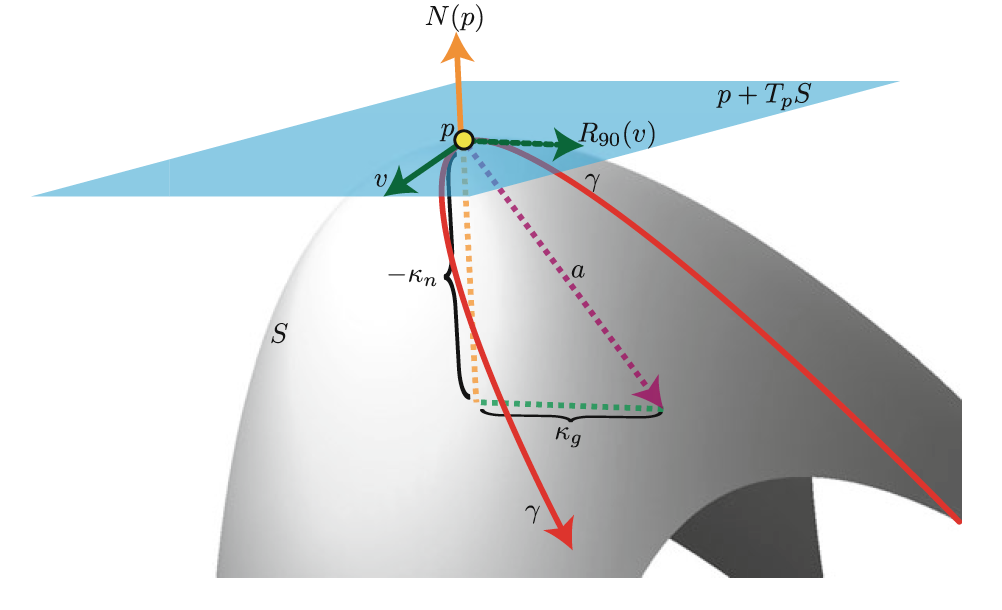
\includegraphics[width=12cm]{./images/normal_and_geodesic_curvature}
    \caption{The normal and geodesic curvature of \(\gamma\) at \(p\)}
    \label{fig:normal_and_geodesic_curvature}
\end{figure}

\begin{definition}[Second Fundamental Form]
    The quadratic form associated with the Weingarten map is called the second fundamental form of \(S\) at \(p\),   and is denoted by the \(\mathbf{II}_p\), i.e.
    \begin{align*}
        \mathbf{II}_p = \left\langle W_p(v), v\right\rangle = \left\langle -dN_p(v), v \right\rangle
    \end{align*}
\end{definition}

\subsection{The Second Fundamental Form in Local Coordinates}
We'll now talk about the second fundamental form in local coordinates as we did with the first fundamental form. Let \( \sigma: U \subset \R^2 \rightarrow S\) be a regular surface patch of S, where \(S\) is a smooth surface, then we define the functions L, M , and N as follows:
\begin{align} \label{eq: define second fundamental form in local coordinates}
    \begin{split}
        L & = \left\langle \sigma_{uu}, N\right\rangle = \left\langle N_u, \sigma_u\right\rangle = { \color{red}\left\langle W(\sigma_u), \sigma_u\right\rangle} \\
        M & = \left\langle \sigma_{uv}, N\right\rangle = - \left\langle N_v, \sigma_u\right\rangle = - \left\langle N_u, \sigma_v\right\rangle  = \left\langle W(\sigma_u), \sigma_v\right\rangle \\
        N & = \left\langle \sigma_{vv}, N\right\rangle = \left\langle N_v, \sigma_v\right\rangle = \left\langle W(\sigma_v), \sigma_v\right\rangle
    \end{split}
\end{align}

These equations are generated u\text{sin}g a similar method to what we did in equation \ref{eq: relating two interpretaion of the normal curvature}. Note that we have suppressed the input variables for brevity. For example, the red term really means that \( L(q) = \left\langle W_{p}(\sigma_u(q)), \sigma_u(q)\right\rangle \), where \(p = \sigma(q)\) and \(q \in U \subset \R^2\). Furthermore, we can represent the second fundamental form in terms of \(E, F, \text{ and } G\) as follows:\\
Suppose \( v \in T_pS\) and \( p \in S\) then,
\begin{align*}
    \mathbf{II}_p(v) & = \mathbf{II}_p(a\sigma_u + b\sigma) = \left\langle W_p(a\sigma_u + b\sigma), a\sigma_u + b\sigma \right\rangle                                                        \\
                     & = a^2 \left\langle W_p(\sigma_u), \sigma_u\right\rangle + 2ab\left\langle W_p(\sigma_u), \sigma_v\right\rangle + b^2\left\langle W_p(\sigma_v), \sigma_v \right\rangle \\
                     & = a^2 E + 2ab F + b^2 G
\end{align*}

This relation motivates the following definition.
\begin{definition}[The Second Fundamental Form in Local Coordinates]
    The second fundamental form in local coordinates \{u,v\} is the expression \[ \mathcal{F}_2 = L du^2 + 2M dudv + N dv^2\]
\end{definition}

As we did in the section \ref{ssec: The first fundamental form in local coordinates} (the first fundamental form in local coordinates), again a good question to ask would be, how reparametrisation of a surface affects the second fundamental form of the surface in terms of the local coordinates?

\begin{example}
    Let a surface patch \( \tilde{\sigma}(\tilde{u}, \tilde{v})\) be a reparametrisation of a surface patch \(\sigma(u,v)\). Assume that \(\Phi: U \rightarrow \tilde{U}\) is a smooth reparametrisation map, then
    \begin{align}
        \begin{pmatrix}
            \tilde{L} & \tilde{M} \\
            \tilde{M} & \tilde{N}
        \end{pmatrix}
        = \pm J(\Phi)^t
        \begin{pmatrix}
            L & M \\
            M & N
        \end{pmatrix}
        J(\Phi)
    \end{align}
\end{example}

\begin{proof}[Proof]
    You would have noticed that the claim here is very similar to the claim in Example \ref{eg: reparmetrisation affect on the first fundamental form} and so is the proof.
    We know
    \begin{align*}
        \tilde{\sigma}_{\tilde{u}}                       & = \sigma_u \frac{\partial u}{\partial \tilde{u}}  + \sigma_v \frac{\partial v}{\partial \tilde{u}}                                                                                                                                                                                                                                                                                                                         \\
        \therefore  \tilde{\sigma}_{\tilde{u} \tilde{u}} & = (\sigma_u \frac{\partial u}{\partial \tilde{u}}  + \sigma_v \frac{\partial v}{\partial \tilde{u}})_{\tilde{u}}                                                                                                                                                                                                                                                                                                           \\
                                                         & = (\sigma_u \frac{\partial u}{\partial \tilde{u}}  + \sigma_v \frac{\partial v}{\partial \tilde{u}})_u \frac{\partial u}{\partial \tilde{u}} +  (\sigma_u \frac{\partial u}{\partial \tilde{u}}  + \sigma_v \frac{\partial v}{\partial \tilde{u}})_v \frac{\partial v}{\partial \tilde{u}}                                                                                                                                 \\
                                                         & = \sigma_{uu} \left(\frac{\partial u}{\partial \tilde{u}} \right)^2 +  \sigma_{uv} \frac{\partial v}{\partial \tilde{u}} \frac{\partial u}{\partial \tilde{u}} + \sigma_u \frac{\partial^2 u}{\partial \tilde{u}^2} + \sigma_{vu} \frac{\partial u}{\partial \tilde{u}}\frac{\partial v}{\partial \tilde{u}} + \sigma_{vv}\frac{\partial^2 v}{\partial \tilde{u}^2} + \sigma_{v} \frac{\partial^2 v}{\partial \tilde{u}^2} \\
        \therefore \tilde{L}                             & = det(J(\Phi))\left( L \left(\frac{\partial u}{\partial \tilde{u}} \right)^2 + 2M \frac{\partial v}{\partial \tilde{u}} \frac{\partial u}{\partial \tilde{u}} + N \left(\frac{\partial v}{\partial \tilde{u}} \right)^2 \right)
    \end{align*}
    This is because \( N\cdot\sigma_u = N\cdot\sigma_v = 0\). Similarly, we can calculate \(\tilde{M} \) and \(\tilde{N}\) in terms of \(N, M, \text{ and } N\). Then as in example \ref{eg: reparmetrisation affect on the first fundamental form} if we represent it in terms of matrices, then we will get the desired result.
\end{proof}

% The normal and geodesic curvature are extrinsic porosities. This means that we can't represent them u\text{sin}g only the first fundamental form.

\section{Gaussian Curvature}
In this section, we'll define two more quantities that measures the curvature of a surface, namely the Gaussian Curvature and Mean Curvature. Gaussian and Mean curvature are dependent on the the following definition:

\begin{definition}[Perincipal Curvature]
    The principal curvature of a surface \( S\) at point \(p\) are the maximum curvature \(\kappa_1\) and minimum curvature \( \kappa_2 \). The directions in which these max \(\kappa_1\) and min curvature \(\kappa_2\) occur are called the principal direction. \\
    Alternatively, the max and min curvature are the eigen values of the Weingarten map \( W_p\) at point \(p \in S\) and the principal direction associated with them are the eigen vectors.
\end{definition}

From the above definition, we can see that we can represent the Weingarten map as a diagonal matrix with a change of basis. Suppose \(v \in T_pS\), where \(|v| = 1\), and let be orthonormal basis be  \( e_1 \) and \( e_2 \) of \( T_pS\). Then, we can represent in \(v\) terms of the basis vectors, i.e. \( v = e_1 \text{cos}(\theta) + e_2 \text{sin}(\theta)\), where \( \theta \) is the angle between \( v\) and \( e_1\).
\begin{align*}
    \mathbf{II}_p(v) & = \left\langle W_p(v), v\right\rangle                                                                              \\
                     & = \left\langle W_p(e_1 \text{cos}(\theta) + e_2 \text{sin}(\theta)), e_1 \text{cos}(\theta) + e_2 \text{sin}(\theta) \right\rangle             \\
                     & = \left\langle e_1 \kappa_1 \text{cos}(\theta) + e_2 \kappa_2 \text{sin}(\theta), e_1 \text{cos}(\theta) + e_2 \text{sin}(\theta)\right\rangle \\
                     & = \kappa_1 \text{cos}(\theta)^2 + \kappa_2 \text{sin}(\theta)^2
\end{align*}

Therefore, if we represent the Weingarten map with respect to the above orthonormal basis then Weingarten map would be:
\begin{align} \label{eq: Weingarten map diagonal matrix}
    W_p = \begin{pmatrix}
        \kappa_1 & 0        \\
        0        & \kappa_2
    \end{pmatrix}
\end{align}
\begin{definition}[Gaussian and Mean Curvature]
    Suppose \(S\) is a regular surface. Let \( W_p: T_pS \rightarrow T_pS \) be the Weingarten map at point \( p \in S\). Then, the Gaussian Curvature (K) is the determinant of the Weingarten map and the Mean curvature (H) is half of the trace. \\
    Alternatively, the Gaussian curvature is also equal to the determinant of the differential \( dN_p: T_pS \rightarrow T_pS \) and the  Mean curvature is also equal to the negative half of the trace of \( dN_p\). This is because the Weingarten map is the same map as the differential \( -dN_p \) with a change of basis.
\end{definition}

We can use equation \ref{eq: Weingarten map diagonal matrix} to write the Gaussian and Mean curvature in the following way:
\begin{align*}
    K = det(W) = \kappa_1\kappa_2 && H = \frac{1}{2} \text{trace}(W) = \frac{\kappa_1 + \kappa_2 }{2}
\end{align*}
\subsection{Gauss Curvature in Local Coordinates}
Now, we will define Gaussian curvature with respect to the local coordinates u\text{sin}g the following proposition:
\begin{proposition}
    Let \( \begin{pmatrix}
        w_{11} & w_{21} \\
        w_{21} & w_{22} 
    \end{pmatrix}\)
    be the matrix that represent the Weingarten map ( \(W_p\) ) at point \( p \in S\) with represent to the basis vectors \{\( \sigma_u, \sigma_v \)\} of \( T_pS \), where \( \sigma: U \rightarrow S\) is a surface patch. Then, 
    \begin{align} \label{eq: Weingarten map local coordinates}
        \begin{pmatrix}
            w_{11} & w_{21} \\
            w_{21} & w_{22} 
        \end{pmatrix} = \frac{1}{EG-F^2} \begin{pmatrix}
            LG - MF & MG - NF \\
            ME - LF & NE- MF
        \end{pmatrix}
    \end{align}
\end{proposition}
\begin{proof}
    U\text{sin}g equation \ref{eg: define second fundamental form in local coordinates} we get the following:
    \begin{align*}
        L & = \left\langle W_p(\sigma_u), \sigma_u \right\rangle = \left\langle w_{11}\sigma_u + w_{21}\sigma_v, \sigma_u\right\rangle = w_{11}E + w_{21}F \\
        M & = \left\langle W_p(\sigma_u), \sigma_v \right\rangle =  \left\langle w_{11}\sigma_u + w_{21}\sigma_v, \sigma_v\right\rangle = w_{11}E + w_{21}G  \\
        M & = \left\langle W_p(\sigma_v), \sigma_u \right\rangle = \left\langle w_{12}\sigma_u + w_{22}\sigma_v, \sigma_u\right\rangle = w_{21}E + w_{22}F  \\
        N & = \left\langle W_p(\sigma_v), \sigma_v \right\rangle = \left\langle w_{12}\sigma_u + w_{22}\sigma_v, \sigma_v\right\rangle = w_{21}F + w_{22}G  
    \end{align*}
\end{proof}
If we represent these equations in a matrix format we get the following: 
\begin{align*}
    \begin{pmatrix}
        w_{11} & w_{21} \\
        w_{21} & w_{22} 
    \end{pmatrix} = 
    \begin{pmatrix}
        E & F \\
        F & G \\
    \end{pmatrix}^{-1}
    \begin{pmatrix}
        L & M \\
        M & N 
    \end{pmatrix}
\end{align*}
It is easy to check that we calculate the inverse then we will get equation \ref{eq: Weingarten map local coordinates}. \\

From this we can get a formula for the Gaussian and Mean curvature in terms the local coordinates. They are as follows:
\begin{align*}
    K & = det(W) = det\left( \frac{1}{EG-F^2} \begin{pmatrix}
        LG - MF & MG - NF \\
        ME - LF & NE- MF
    \end{pmatrix} \right) = \frac{LN-M^2}{EG-F^2} \\
    H & = \text{trace}(W) = \text{trace}\left(\frac{1}{EG-F^2} \begin{pmatrix}
        LG - MF & MG - NF \\
        ME - LF & NE- MF
    \end{pmatrix} \right) = \frac{LG-2MF+NE}{2(EG-F^2)}
\end{align*}

In order to fully understand these concepts, we'll consider the following examples:

\begin{example} \label{eg: Gaussian curvature of surface of revolution}
    In this example, we'll calculate the Gaussian curvature for a general surface of revolution. A surface of revolution is obtained by rotating a plane curve, called the profile curve, around a straight line in the plane. Suppose \( \gamma(u) = (f(u),0,g(u))\) is a parametrisation of a profile curve in the \{x, z\} plane and let \( \sigma(u,v) = (\text{cos}(v)f(u), \text{sin}(v)f(u), g(u) )\) be the surface obtained by rotating the profile around the \(z\) axis. Then, 
    \begin{align*}
        \sigma_u & = (\text{cos}(v)f^{\prime}, \text{sin}(v)f^{\prime}, g^{\prime} ) \\
        \sigma_v & = (-\text{sin}(v)f, \text{cos}(v)f, 0) \\
        \therefore \; \; & \sigma_u \times \sigma_v = (-\text{cos}(v)fg^{\prime} , -\text{sin}(v)fg^{\prime}, f^{\prime} f) \\
        \therefore \; \; &  \left\lVert\sigma_u \times \sigma_v \right\rVert = \sqrt{(fg^{\prime})^2 + (ff^{\prime})^2} = \sqrt{f^2((g^{\prime})^2 + (f^{\prime})^2)}
    \end{align*} 
    Therefore, \( \left\lVert\sigma_u \times \sigma_v \right\rVert \) will be non-vanishing if \( f \) is never \(0\), this means the profile curve never intersect the z axis, and \(  (g^{\prime})^2 + (f^{\prime})^2 \neq 0 \), this means the profile curve is regular. We know if a curve is regular, then there exists a reparametrisation of this curve such that its reparametrisation is unit speed; therefore, we might as well assume that the profile curve is unit-speed. \\
    To calculate the Gaussian curvature, we must first calculate the first and the second fundamental form in terms of the local coordinates. \\
    The first fundamental form in local coordinates: 
    \begin{align*}
        E & = \left\langle \sigma_u , \sigma_u\right\rangle  = \left\lVert (\text{cos}(v)f^{\prime}, \text{sin}(v)f^{\prime}, g^{\prime} ) \right\rVert^2 = (f^{\prime})^2 + (g^{\prime})^2  = 1 \\
        F & = \left\langle \sigma_u, \sigma_v \right\rangle = \left\langle (\text{cos}(v)f^{\prime}, \text{sin}(v)f^{\prime}, g^{\prime} ), (-\text{sin}(v)f, \text{cos}(v)f, 0 ) \right\rangle = 0 \\
        G & = \left\langle \sigma_v, \sigma_v \right\rangle  = \left\lVert (-\text{sin}(v)f, \text{cos}(v)f, 0) \right\rVert ^2 = f^2
    \end{align*}
    The Gaussian Map in local coordinates:
    \begin{align*}
        N = \frac{\sigma_u \times \sigma_v }{\left\lVert \sigma_u \times \sigma_v \right\rVert } & =  \frac{\left( -\text{cos}(v)g^{\prime}f, -\text{sin}(v)g^{\prime}f, ff^{\prime} )\right)}{f} \text{  (  because  \((f^{\prime})^2 + (g^{\prime})^2  = 1  ) \)} \\ 
        & = \left( -\text{cos}(v)g^{\prime}, -\text{sin}(v)g^{\prime}, f^{\prime} \right)
    \end{align*}
    The second fundamental form in local coordinates:
    \begin{align*}
        \sigma_{uu} & = (\text{cos}(v)f^{\prime \prime}, \text{sin}(v)f^{\prime \prime}, g^{\prime \prime}) \\
        \sigma_{uv} & = (-\text{sin}(v)f^{\prime}, \text{cos}(v)f^{\prime}, 0) \\
        \sigma_{vv} & = (-\text{cos}(v)f, -\text{sin}(v)f, 0 ) \\
        \therefore \; \; \; \; L & = \left\langle \sigma_{uu}, N \right\rangle = g^{\prime \prime}f^{\prime} -  f^{\prime \prime} g^{\prime}\\
        M & = \left\langle \sigma_{uv} , N \right\rangle = 0 \\
        N & = \left\langle \sigma_{vv} , N \right\rangle = fg^{\prime} 
    \end{align*}
    Therefore, the Gaussian curvature equals the following:
    \begin{align*}
        K = \frac{LN-M^2}{EG-F^2}  & = \frac{(g^{\prime \prime}f^{\prime} -  f^{\prime \prime} g^{\prime})(fg^{\prime} ) }{ f^2} \\
         & =  \frac{(g^{\prime \prime}f^{\prime} -  f^{\prime \prime} g^{\prime})(g^{\prime} ) }{ f} \\
         & = \frac{-f^{\prime \prime}}{f}
    \end{align*}
     This is because of the following:
     \begin{align*}
        (f^{\prime})^2 + (g^{\prime})^2  = 1  \implies f^{\prime}f^{\prime \prime} + g^{\prime}g^{\prime \prime}  = 0 \\
        \shortintertext{Then, }
        (g^{\prime \prime}f^{\prime} -  f^{\prime \prime} g^{\prime})(g^{\prime} ) & = g^{\prime \prime}f^{\prime}g^{\prime}  -  f^{\prime \prime} (g^{\prime})^2 \\
        & =  -f^{\prime \prime}(f^{\prime})^2  -  f^{\prime \prime} (g^{\prime})^2 \\
        & = -f^{\prime \prime}
     \end{align*}
\end{example}

Now, a good question to ask would be that if the Gaussian curvature is given can we find a surface that has the given Gaussian curvature? For simplicity, we will assume that the Gaussian curvature is constant for the entire surface; however, before we do this, we need to consider the following example:

\begin{example}
    Show that when we apply a dilation \( (x,y,z) \rightarrow a(x,y,z) \), where \(a\) is a non-zero constant, on a surface its Gaussian curvature gets multiplied by \(a^{-2}\).
\end{example}
\begin{proof}
    Suppose \( S \) is a surface and \(\sigma: U \rightarrow S \) is a surface patch of \(S\). Let \(K\) be the Gaussian curvature of S, \( \tilde{\sigma} = a\sigma \) and let \( Fdu^2 + 2Gdudv + Hdv^2 \) be the first fundamental form and \( Ldu^2 + 2Mdudv + Ndv^2 \) be the second fundamental form of \(S\). \\
    Then the first fundamental form of \( \tilde{\sigma}\) is :
    \begin{align*}
        \tilde{E} & = \left\langle \tilde{\sigma}_u, \tilde{\sigma}_u \right\rangle = \left\langle a\sigma_u, a\sigma_u \right\rangle = a^2 \left\langle \sigma_u, \sigma_u \right\rangle = a^2 E \\
        \tilde{F} & = \left\langle \tilde{\sigma}_u, \tilde{\sigma}_v \right\rangle = \left\langle a \sigma_u, a \sigma_v \right\rangle = a^2 \left\langle \sigma_u, \sigma_v \right\rangle = a^2 F \\
        \tilde{G} & = \left\langle \tilde{\sigma}_v, \tilde{\sigma}_v \right\rangle = \left\langle a\sigma_v, a\sigma_v \right\rangle = a^2 \left\langle \sigma_v, \sigma_v \right\rangle = a^2 G 
    \end{align*}
    The Normal of \( \tilde{\sigma}\) is: 
    \begin{align*}
        \tilde{N} = \frac{\tilde{\sigma}_u \times  \tilde{\sigma}_v}{\left\lVert \tilde{\sigma}_u \times  \tilde{\sigma}_v\right\rVert } = \frac{a^2 (\sigma_u \times \sigma_v) }{ \left\lVert a^2 (\sigma_u \times \sigma_v) \right\rVert } = N
    \end{align*}
    The second fundamental form of \( \tilde{\sigma}\) is:
        \begin{align*}
            \tilde{L} & = \left\langle \tilde{\sigma}_{uu}, \tilde{N} \right\rangle = \left\langle a \sigma_{uu}, N \right\rangle = aL \\
            \tilde{M} & = \left\langle \tilde{\sigma}_{uv}, \tilde{N} \right\rangle = \left\langle a \sigma_{uv}, N \right\rangle = aM \\
            \tilde{N} & = \left\langle \tilde{\sigma}_{vv}, \tilde{N} \right\rangle = \left\langle a \sigma_{vv}, N \right\rangle = aN 
        \end{align*}
        Therefore, the Gaussian curvature of the surface after dilation is:
        \begin{align*}
            \tilde{K} = \frac{\tilde{L}\tilde{N} - \tilde{M}^2}{\tilde{E}\tilde{G}-\tilde{F}^2} = \frac{a^2 (LN-M^2) }{ a^4( EG-F^2)} = \frac{K}{a^2}
        \end{align*}
\end{proof}
From the above example, we can tell that we only need to consider 3 cases, when the Gaussian curvature is -1, 0, and 1. This is because we can get all the other Gaussian curvatures by just a dilation of the surface.

\begin{example}
    Suppose that the given Gaussian curvature is -1. Then, u\text{sin}g the same format as in example \ref{eg: Gaussian curvature of surface of revolution}, we know that \( -1 = \frac{-f^{\prime \prime}}{f}\), i.e. \( f = f^{\prime \prime} \). Then, the general solution is \( f(u) = ae^u + be^{-u}\), where \( a,b \in \R \). For simplicity, let \( f(u) = e^u \) then,
    \begin{align*}
        & (f^\prime)^2 + (g^\prime)^2 = 1 \implies g^\prime = \pm \sqrt{1-(f^\prime)^2} = \pm \sqrt{1-e^{2u}}
        \shortintertext{This implies}
        g(u) & = \int \sqrt{1-e^{2u}} du = \sqrt{1-e^{2u}} - \text{\text{cos}h}^{-1}(e^{-u}) 
    \end{align*}
    The evaluation of this integral has been left as an exercise for the reader. We dropped the \( \pm\) sign as we are only looking for one possible surface. Therefore, a surface with Gaussian curvature -1 is 
    \begin{align*}
        \sigma(u,v) & = (\text{cos}(v)f(u), \text{sin}(v)f(u), g(u)) \\
         & = (\text{cos}(v) e^u, \text{sin}(v) e^u , \sqrt{1-e^{2u}} - \text{\text{cos}h}^{-1}(e^{-u})  )
    \end{align*}
    If we were to consider the general case then the general function would be the following:
    \begin{align*}
        \sigma(u,v) = \left(\text{cos}(v) (ae^u + be^{-u}), \text{sin}(v) (ae^u + be^{-u}), \int \pm \sqrt{1-(ae^u - be^{-u})^2} \right) 
    \end{align*}
\end{example}

\begin{example}
    Suppose that the given Gaussian curvature is 0. Then, using the same format as in example \ref{eg: Gaussian curvature of surface of revolution}, we know \( 0 = \frac{-f^{\prime \prime}}{f} \), i.e. \( f^{\prime \prime} = 0\). This implies that \( f(u) = au \),  where \( a \in \R \). Then,
    \begin{align*}
        (f^\prime)^2 + (g^\prime)^2 = 1 \implies g^\prime = \pm \sqrt{1-(f^\prime)^2} = \pm \sqrt{1 - a^2}
        \shortintertext{Therefore, }
        g = \pm \int \sqrt{1 - a^2} du = \pm (\sqrt{1 - a^2})u + c \\
        \shortintertext{Hence, }
        \sigma(u,v) = (a \; \text{cos}(v)u, a \; \text{sin}(v) u, bu + c)
        \shortintertext{, where \(b = \pm \sqrt{1 - a^2} \)}
    \end{align*}
\end{example}
\begin{example}
    Suppose the given Gaussian curvature is 1. Then, using the same formula as in example \ref{eg: Gaussian curvature of surface of revolution}, we know \( 1 = \frac{-f^{\prime \prime}}{f} \), i.e. \( f = -f^{\prime \prime }\). Then, the general solution is \( f(u) =  a \; \text{sin}(u) + b \; \text{cos}(u) \), where \( a,b \in \R \). Then,

    \begin{align*}
        (f^\prime)^2 + (g^\prime)^2 & = 1 \implies g^\prime = \pm \sqrt{1-(f^\prime)^2} = \pm \sqrt{1 - (a \; \text{cos}(u) - b \; \text{sin}(u) )^2 } \\
        \shortintertext{This implies }
        g(u) & = \pm \int \sqrt{1 - (a \; \text{cos}(u) - b \; \text{sin}(u))^2  }
    \end{align*}
    For simplicity, lets assume that \( f(u) = \text{sin}(u)\) and \( g(u) = \int \sqrt{1 - (\text{cos}(u))^2 } = \int \text{sin(}u) du = cos(u) + c\). Therefore, a surface with Gaussian calculate 1 is
    \begin{align*}
        \sigma(u,v) =  ( \text{cos}(v)\text{sin}(u), \text{sin}(v) \text{sin}(u), \text{cos}(u))
    \end{align*}
    , which is a unit sphere. If we were to consider the general case then the general function would be the following:
    \begin{align*}
        \sigma(u,v) = \left(\text{cos}(v) ( a \; \text{sin}(u) + b \; \text{cos}(u) ) , \text{sin}(v) ( a \; \text{sin}(u) + b \; \text{cos}(u)) , \pm \int \sqrt{1 - (a \; \text{cos}(u) - b \; \text{sin}(u))^2  }  \right)
    \end{align*}
\end{example}

    {\color{red}
        - Example \checkmark \\
        - Gaussian Curvature , Give the formula show what gaussian curves is equal to w.r.t. the first and second fundamental form. \checkmark\\
        - Example that Pedram asked \checkmark \\
        - Gauss Bonnet Theorem \ding{55}}
        \end{document}

